
\newpage

\section{Large Language Models}

    I Large Language Models (LLM) condividono il principio di base dei modelli n-gram: assegnano probabilità a sequenze di parole e generano testo campionando la parola successiva. Tuttavia, a differenza dei modelli basati su conteggi, gli LLM sono reti neurali addestrate su enormi quantità di testo per indovinare il token successivo, apprendendo implicitamente molta conoscenza linguistica e fattuale.

    \subsection{Architetture}

        Esistono tre principali tipologie di architetture per gli LLM:
        \begin{enumerate}
            \item \textbf{Decoders (Decoder-only)}: Noti anche come Causal o Autoregressive LLMs. Predicono le parole da sinistra a destra (es. GPT, Llama, Claude).
            \item \textbf{Encoders (Encoder-only)}: Come i Masked Language Models visti in precedenza (famiglia BERT). Usati principalmente per classificazione, predicono parole basandosi sul contesto sia destro che sinistro.
            \item \textbf{Encoder-Decoders}: Mappano una sequenza in un'altra. Popolari per traduzione automatica e summarization (es. Flan-T5, BART).
        \end{enumerate}

    \subsection{Decoder-only Models e Conditional Generation}

        Concentriamoci sui modelli \textbf{Decoder-only}. Questi modelli eseguono una "generazione condizionata": generano testo condizionato dal testo precedente (prefix o prompt).

        Molti task NLP pratici possono essere riformulati come problemi di predizione della parola successiva (Word Prediction):
        \begin{itemize}
            \item \textbf{Sentiment Analysis}: "The sentiment of the sentence 'I like Jackie Chan' is:" $\rightarrow$ il modello predice "positive".
            \item \textbf{Question Answering}: "Q: Who wrote The Origin of Species? A:" $\rightarrow$ il modello predice "Charles".
            \item \textbf{Summarization}: Si fornisce il testo originale seguito da un token speciale come "tl;dr" e il modello genera il riassunto.
            \begin{figure}[H]
                \centering
                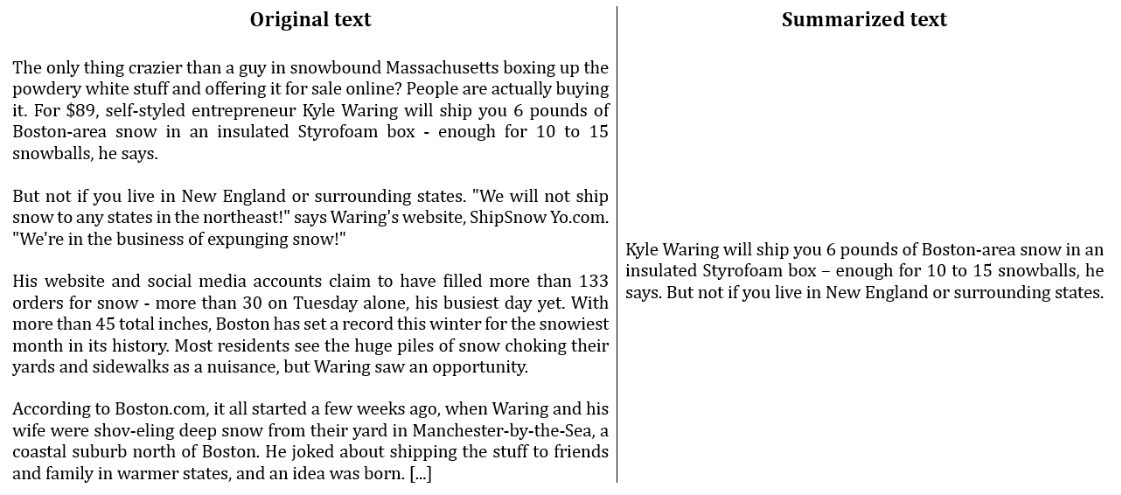
\includegraphics[width=0.9\linewidth]{imgs/schema_8_1.png}
                \label{fig:fig81}
            \end{figure}
        \end{itemize}

    \newpage

    \subsection{Decoding e Strategie di Campionamento}

        Il \textit{decoding} è il processo di scelta della parola da generare basandosi su un criterio applicato alle probabilità fornite in output dal modello. I layer neurali degli LLM generano un vettore di logit $u$, che viene trasformato in una distribuzione di probabilità $y$ tramite la funzione softmax. Le strategie di decodifica si dividono in due grandi famiglie: \textbf{deterministiche} e \textbf{stocastiche}.

        \subsubsection{Decoding Deterministico}
            Queste strategie effettuano scelte prevedibili massimizzando le probabilità, ma i testi generati tendono a risultare ripetitivi e poco interessanti.

            \paragraph{Greedy Search}
            È il metodo di decodifica più semplice: fornisce ad ogni passo la scelta localmente migliore, selezionando la parola con la probabilità più alta. Formalmente, il token generato è:
            $$w_t = \text{argmax}_w P(w|w_{1:t-1})$$
            
            \begin{figure}[H]
                \centering
                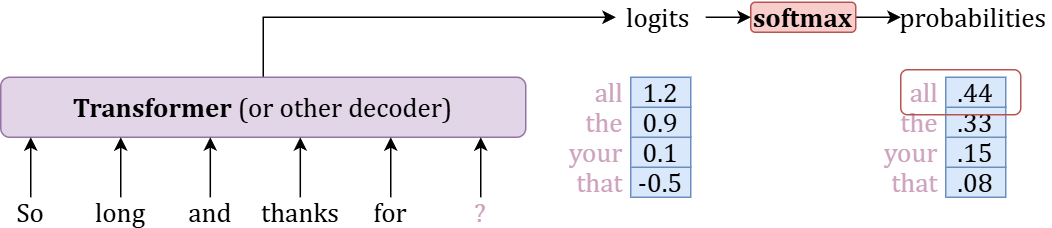
\includegraphics[width=0.6\linewidth]{imgs/schema_8_2.png}
                \label{fig:fig82}
            \end{figure}
            
            Il limite principale di questo algoritmo è che può produrre frasi ripetitive e non sempre garantisce il risultato globale migliore, poiché potrebbe scartare percorsi ottimali nascosti dietro un token con probabilità localmente bassa.

            \paragraph{Beam Search}
            Questo algoritmo riduce il rischio di perdere sequenze di parole con probabilità globalmente elevata mantenendo in memoria un numero fisso di ipotesi candidati, definito dal parametro $num\_beam$. Ad ogni passo, esplora le continuazioni delle ipotesi correnti e seleziona le $num\_beam$ sequenze con la probabilità cumulativa maggiore. Quando $num\_beam = 1$, l'algoritmo coincide esattamente con la greedy search.

            \begin{figure}[H]
                \centering
                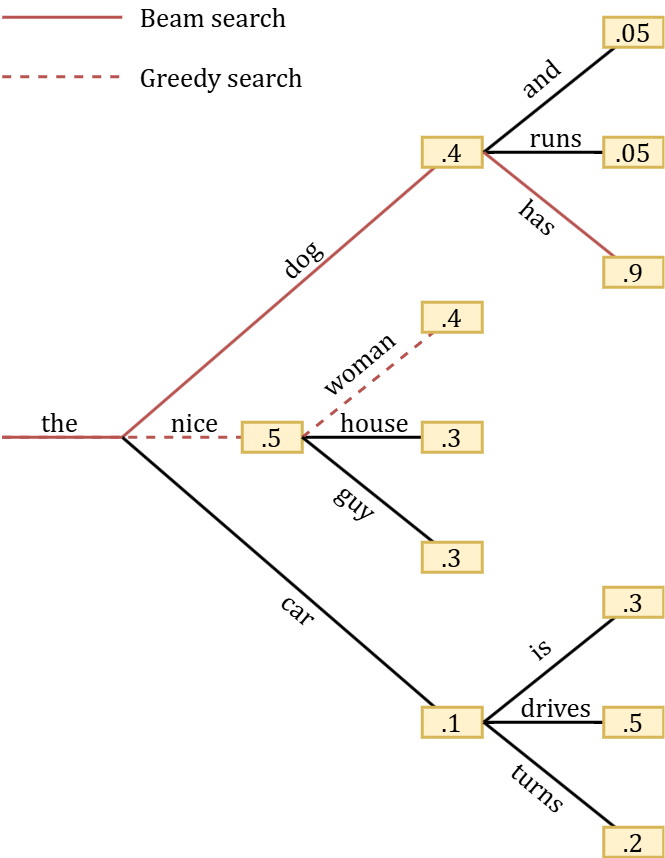
\includegraphics[width=0.4\linewidth]{imgs/schema_8_3.png}
                \label{fig:fig83}
            \end{figure}

        \subsubsection{Decoding Stocastico (Sampling)}
            Per superare la ripetitività dei metodi deterministici si introduce un elemento randomico, campionando i token da una distribuzione. Questa famiglia di metodi richiede di bilanciare un compromesso: favorire i token più probabili aumenta la qualità (testi accurati, coerenti e fattuali), mentre esplorare token a media probabilità migliora la diversità e creatività, a rischio però di minore coerenza (allucinazioni).

        \paragraph{Random (Multinomial) Sampling}
        Il token successivo viene selezionato in modo casuale, ma in misura proporzionale alla sua probabilità calcolata dal modello rispetto alle scelte precedenti: $w_i \sim p(w_i|w_{<i})$. Poiché anche le parole strane o fuori contesto mantengono una piccola probabilità, sommate costituiscono una fetta rilevante della distribuzione (la "coda lunga") che, se campionata, porta a frasi senza senso.

        \paragraph{Top-k Sampling}
        Per escludere la coda lunga, questa tecnica imposta un limite $k$ fisso. Il modello calcola la \textit{likelihood} di ogni parola nel vocabolario e mantiene solo le $k$ parole più probabili. I punteggi di queste parole vengono poi rinormalizzati in una distribuzione di probabilità valida dalla quale si campiona casualmente. Il limite di questa strategia è la rigidità: avendo $k$ fisso, copre quantità molto diverse di massa di probabilità a seconda che la distribuzione del modello in un certo contesto sia piatta o molto piccata.

        \paragraph{Top-p (Nucleus) Sampling}
        Invece di un numero fisso di candidati, si mantiene fissa la massa di probabilità totale per implementare una selezione adattiva (un valore di $k$ dinamico). Dato il contesto, il vocabolario candidato $V^{(p)}$ è l'insieme più piccolo di parole la cui somma delle probabilità raggiunge una determinata soglia $p$:
        $$\sum_{w \in V^{(p)}} P(w|w_{<t}) \ge p$$

        \paragraph{Temperature Sampling}
        Questa tecnica non tronca l'insieme dei candidati, ma ne rimodella la distribuzione sfruttando l'iperparametro di temperatura $\tau$. Il vettore dei logit $u$ viene diviso per $\tau$ prima di essere passato alla funzione softmax:
        $y = \text{softmax}(u/\tau)$.
        \begin{itemize}
            \item $\tau < 1$ (\textit{Low temperature}): Spinge verso 1 i valori alti e verso 0 i valori bassi, enfatizzando i token più probabili e comportandosi in maniera più "greedy".
            \item $\tau \to 1$: La distribuzione originale rimane sostanzialmente invariata.
            \item $\tau > 1$ (\textit{High temperature}): Il sistema diventa più "caldo" e flessibile, la distribuzione si appiattisce tendendo a quella uniforme, esplorando più combinazioni possibili.
        \end{itemize}

        \paragraph{Contrastive Search}
        Questa strategia avanzata mira a generare token che siano al contempo probabili per il modello e discriminativi rispetto al contesto precedente. Il token $x_t$ è selezionato dai top-$k$ candidati bilanciando la probabilità intrinseca (\textit{model confidence}) con una penalità di degenerazione che sfrutta la \textit{cosine similarity} ($s$) degli embedding:
        $$x_t = \arg\max_{v \in V^{(k)}} \left\{ (1-\alpha) \times \frac{p_\theta(v|x_{<t})}{\text{model confidence}} - \alpha \times (\max \{s(h_v, h_{x_j}): 1 \le j \le t-1\}) \right\}$$
        L'iperparametro $\alpha$ regola il peso di queste componenti: aumentando $\alpha$, il token si discosta maggiormente dal contesto precedente; se $\alpha = 0$, la ricerca degenera nella semplice greedy search.

    \newpage

    \subsection{Pre-training}

        L'algoritmo di training è \textbf{Self-supervised}: l'etichetta (label) è semplicemente la parola successiva nel testo.
        Si utilizza la \textbf{Cross-Entropy Loss}:
        $$ L_{CE} = - \sum_{w \in V} (y_t[w]) \log(\hat{y}_t[w]) = - \log \hat{y}_t[w_{t+1}] $$
        Dove $w_{t+1}$ è la parola corretta successiva.

        Durante il training si usa il \textbf{Teacher Forcing}: al passo $t+1$, il modello riceve in input la parola corretta $w_{t+1}$ (ground truth) e non quella che ha predetto al passo precedente.

        \subsubsection{Dati di Pre-training}
            I modelli sono addestrati su enormi porzioni del web (es. Common Crawl, C4, The Pile).
            È necessario filtrare i dati per qualità (rimuovere boilerplate, deduplicazione) e sicurezza (tossicità, PII - Personally Identifiable Information).
            Rimangono aperti problemi legali legati al copyright e al "Fair Use".

    \subsection{Fine-Tuning dei LLM}

        Il \textit{fine-tuning} è il processo mediante il quale un modello pre-addestrato (Foundation Model) viene sottoposto ad ulteriori iterazioni di addestramento su nuovi dati specifici, al fine di adattarlo a un particolare dominio (es. medico, legale, finanziario) o a task specifici.

        Esistono diverse tipologie e strategie per effettuare il fine-tuning di un LLM:
        \begin{itemize}
            \item Aggiunta di una \textbf{Head} (classificatore) in cima al modello.
            \item \textbf{Continued Pretraining}: si continua ad addestrare tutto il modello su nuovi dati con la stessa loss.
            \item \textbf{Supervised Finetuning (SFT)}: per instruction tuning (dataset di prompt-risposta).
        \end{itemize}

        \subsubsection{Parameter-Efficient Fine Tuning (PEFT)}
            Riapplicare il training a tutti i parametri del modello (\textit{full fine-tuning}) è un'operazione estremamente lenta e costosa dal punto di vista computazionale. 
            Le tecniche PEFT superano questo ostacolo congelando la maggior parte dei pesi pre-addestrati e aggiornando solo un piccolo sottoinsieme di parametri (spesso solo negli ultimi layer) in modo efficiente.

    \subsection{Valutazione dei LLM}

        Le prestazioni dei Large Language Models vengono misurate secondo diversi criteri:
        \begin{itemize}
            \item \textbf{Accuracy} e \textbf{Metriche Task-Oriented}: Come F1-Score, BLEU, ROUGE.
            \item \textbf{Costi e Prestazioni}: Velocità di esecuzione ed efficienza energetica (es. kWh consumati, emissioni $CO_2$).
            \item \textbf{Fairness (Equità)}: Valutazione della presenza di bias interni o stereotipi di genere/razziali generati.
        \end{itemize}

        \subsubsection{Log-Likelihood e Perplexity}
            Poiché i modelli generano testo in base alla probabilità congiunta, potremmo confrontare i modelli usando la \textit{log-likelihood}. Tuttavia, essa diminuisce all'aumentare della lunghezza del testo. 
            
            La metrica per valutare i LM è la \textbf{Perplexity} (inverso della probabilità normalizzata per la lunghezza):
            $$ PP(W) = \sqrt[n]{\prod_{i=1}^n \frac{1}{P(w_i | w_{<i})}} $$
            Minimizzare la perplessità equivale a massimizzare la probabilità del test set.

            È importante notare che la perplexity è sensibile al processo di tokenizzazione; per confrontare due modelli diversi è necessario che utilizzino lo stesso tokenizer.

    \subsection{Scalabilità e Tecniche di Ottimizzazione}

        La scalabilità dei modelli è studiata per comprendere come migliorare le performance e come gestire LLM con centinaia di miliardi di parametri (come Llama 3.1 405B) in scenari con risorse limitate.

    \subsection{Leggi di Scaling (Scaling Laws)}
        Le prestazioni di un LLM (misurate tramite la loss $L$) scalano secondo una legge di potenza rispetto a tre fattori principali (mantenendo costanti gli altri):
        \begin{enumerate}
            \item Dimensione del modello ($N$): $L(N) = (\frac{N_c}{N})^{\alpha_N}$
            \item Dimensione del dataset ($D$): $L(D) = (\frac{D_c}{D})^{\alpha_D}$
            \item Budget di computazione ($C$): $L(C) = (\frac{C_c}{C})^{\alpha_C}$
        \end{enumerate}
        Queste equazioni empiriche permettono di stimare la loss finale già all'inizio del training.

        Il numero di parametri non-embedding $N$ può essere approssimato come:
        $N \approx 12 \cdot n_{layer} \cdot d^2$ 
        (assumendo $d_{attn} = d_{ff}/4 = d$).

        \subsubsection{KV Cache}
            Mentre durante il training la self-attention viene calcolata efficientemente in parallelo tramite $A = \text{softmax}(\frac{QK^\top}{\sqrt{d_k}})V$, in fase di inferenza la generazione è autoregressiva (un token alla volta).

            Per evitare di ricalcolare le matrici Key ($K$) e Value ($V$) per tutti i token generati in precedenza $X_{<j}$, questi vettori vengono memorizzati in una struttura chiamata \textbf{KV Cache}, permettendo al modello di recuperarli direttamente per i passaggi successivi, riducendo drasticamente il costo computazionale.

        \subsubsection{LoRA (Low-Rank Adaptation)}
            LoRA è una popolare tecnica PEFT usata per ottimizzare il fine-tuning. Nei layer di self-attention ci sono grandi matrici di pesi densi ($W \in \mathbb{R}^{d \times d}$). Invece di aggiornare l'intera matrice ($W \rightarrow W + \Delta W$), LoRA congela i pesi originali e apprende solo un aggiornamento approssimato a basso rango (\textit{Low-Rank}) tramite la decomposizione in due matrici $A$ e $B$:
            \begin{itemize}
                \item $A \in \mathbb{R}^{N \times r}$
                \item $B \in \mathbb{R}^{r \times d}$
            \end{itemize}
            con il rango $r \ll \min(N,d)$. 
            Durante il \textit{forward pass}, l'operazione diventa quindi:
            $h = xW + xAB$
            Il numero di parametri aggiornabili diventa minuscolo, abbattendo drasticamente l'uso di memoria VRAM.

        \subsubsection{Quantizzazione}
            I parametri dei modelli sono convenzionalmente salvati nel formato floating point a 32-bit (FP32). La quantizzazione è una tecnica di compressione che riduce la precisione con cui i pesi vengono salvati (ad esempio a FP16, FP8 o interi INT8), in modo da ridurre notevolmente lo spazio occupato in memoria e accelerare l'inferenza, con una perdita marginale in termini di performance.